\documentclass[12pt]{article}

\usepackage{fullpage}
\usepackage{multicol,multirow}
\usepackage{tabularx}
\usepackage{ulem}
\usepackage[utf8]{inputenc}
\usepackage[russian]{babel}
\usepackage{color} %% это для отображения цвета в коде
\usepackage{listings} %% собственно, это и есть пакет listings
\usepackage{graphicx}%Вставка картинок правильная
\usepackage{float}%"Плавающие" картинки
\usepackage{wrapfig}%Обтекание фигур (таблиц, картинок и прочего)
\usepackage{caption}
\lstloadlanguages{C}
\parindent=1cm
\DeclareCaptionFont{white}{\color{white}} %% это сделает текст заголовка белым
%% код ниже нарисует серую рамочку вокруг заголовка кода.
\DeclareCaptionFormat{listing}{\colorbox{gray}{\parbox{\textwidth}{#1#2#3}}}
\captionsetup[lstlisting]{format=listing,labelfont=white,textfont=white}

\begin{document}

\section*{Лабораторная работа №\,3 по курсу Криптография}

Выполнила студентка группы 08-307 МАИ \textit{Усачева Елизавета}.

\subsection*{Задание}
Сравнить:
\begin{itemize}
    \item Два осмысленных текста на естественном языке.
    \item Осмысленный текст и текст из случайных букв.
    \item Осмысленный текст и текст из случайных слов.
    \item Два текста из случайных букв.
    \item Два текста из случайных слов.
\end{itemize}
Как сравнивать: считать процент совпадения букв в сравниваемых текстах – получить дробное значение от 0 до 1 как результат деления количества совпадений на общее число букв. Расписать подробно в отчёте алгоритм сравнения и приложить сравниваемые тексты в отчёте хотя бы для одного запуска по всем пяти подпунктам. Осознать какие значения получаются в этих пяти подпунктах. Привести свои соображения о том почему так происходит.\\
\\
Длина сравниваемых текстов должна совпадать. Привести соображения о том какой длины текста должно быть достаточно для корректного сравнения.

\subsection*{Введение}

Открытый текст — в криптографии исходный текст, подлежащий шифрованию, либо получившийся в результате расшифровки. Может быть прочитан без дополнительной обработки.
\\
Заменив реальный открытый текст его моделью, можно построить критерий распознавания открытого текста. При этом можно воспользоваться либо стандартными методами различения статистических гипотез, либо наличием в открытых текстах некоторых запретов, таких, например, как биграмма ЪЪ в русском тексте.

\subsection*{Метод решения}
\subsubsection*{Способ сранвения}
Я решила сравнивать "наивно". Т.е. я просто подсчитываю процент совпадения символов на соответсвующих местах в двух разных текстах. Алгоритм подсчета реализован в файле {\it comparing.c}:
\lstset{language=C}
\begin{lstlisting}
while (buff1[i] != '\0' && buff2[i] != '\0')
{
if (buff1[i] == buff2[i])
	res++;
	i++;
}
res = res / n;
\end{lstlisting}
\subsubsection*{Генерация текстов}
Механизмы генерации текстов (осмысленных, из случайных букв, из случайных слов) описаны в файлах {\it generate.c}, {\it generate\_random\_words.py}.
\\
За основу для осмысленных текстов был взят роман "Гордость и предубеждение" Джейн Остин. Я "нарезала" кусочки нужно мне длины. Для текстов, состоящих из случайных букв, я просто использовала рандомное размещение букв различного регистра. Также были сгенерированы тексты различной длины. Генерация текстов из случайных слов производилась из заранее скачанного словаря, затем этот словарь был преобразован в массив и далее процесс генерации был схож с процессом генерации текста из случайных букв, только в данном случае буквами были слова из массива.

\subsection*{Результат работы:}
\begin{figure}[h]
    \centering
    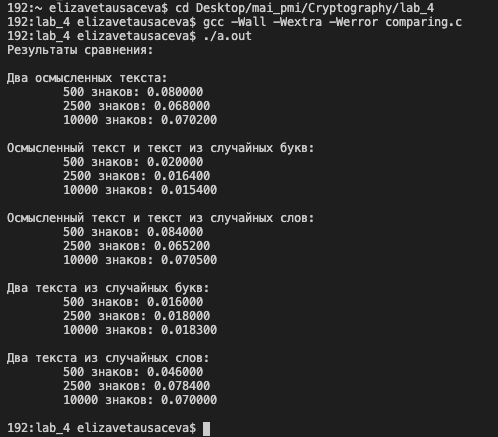
\includegraphics[width=0.5\linewidth]{1.png}
\end{figure}

\subsection*{Выводы}
Первый вывод, который можно сделать, это то, что чем больше объем текста, тем точнее будет статистика. Однако, нет смысла увеличивать объем текста до бесконечности, т.к. определенную закономерность можно выявить на относительно небольшой выборке. В текстах из случайных букв этой закономерности вообще заведомо нет, так что в этом тоже можно обойтись небольшой выборкой. Наиболее подходящим объемом выглядит текст, содержащий примерно 5000-10000 знаков.\\
Наиболее высокую вероятность совпадения мы видим в сравнении двух осмысленных текстов, осмысленного текста и текста из случайных слов, двух текстов из случайных слов. Это связано с тем, что при таком способе сравнения никак не учитываются смысловые конструкции и контекст, которые присутсвуют в осмысленных текстах, но отсутствуют в текстах из случайных слов.\\
Сравнивая два текста из случайных букв мы получаем велечину примерно равную вероятности выпадения случайной буквы из алфавита (в разных регистрах).Это объясняется тем, что в текстах, состоящих их случайных букв, сгенерированных мной, нет ни знаков пробелов, табуляции, переноса строки и знаков препинания. \\
Однако, можно увидеть существенную разницу в сравнениях двух осмысленных текстов и одного осмысленного и одного текста из случайных букв. Конечно, в осмысленных текстах есть буквы, которые используются чаще ("а", например) и есть буквы, которые используются реже ("ъ", например). Однако, при сравнении осмысленного текста и текста, состоящего из случайных букв, вероятность совпадения будет примерно такая же, как если бы мы сравнивали два текста, состоящих из случайных букв, ведь во втором случае нет таких вариантов, которые попадались бы чаще или реже, чем другие. Поэтому здесь появляется проблема случайного пропуска осмсленного текста. Т.е. если мы захотим выбрать из пары текстов осмысленный, то в такой комбинации мы пропустим осмысленный текст посчитав, что выбрали два текста из случайных букв. Та же проблема будет в парах: текст из случайных слов-осмысленный текст и два текста из случайных букв. Здесь наоборот можно принять текст из случайных слов за осмысленный текст.\\
Главной причиной таких ошибок я считаю сам способ сравнения. Он не учитывает контекста, не учитывает хотя бы наличие знаков препинания, буквосочетаний определенных и пр. 

\end{document}

